%\documentclass{article}
%\usepackage{graphicx,subfigure}
%\begin{document}

\begin{figure}[!h]
  \centering
  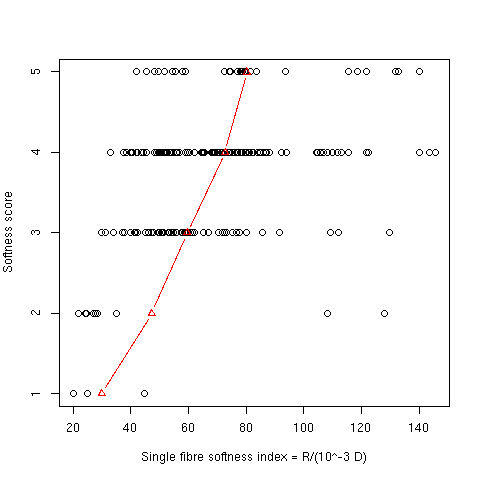
\includegraphics[width=0.9\textwidth]{soft.png}
  \caption{Plot of Softness Index $(I)$ calculated as $R/(10^{-3} D$ against subjective Softness Scores done on wool staples, for 340 Merino sheep in a data set belonging to Dr Jim Watts. The $R$ refers to intrinsic radius of curvature in $mm$ calculated from follicle curvature scores as described in Jackson and Watts(2016)~\cite{jack:16b}, and the $D$ refers to average fibre diameter in microns. The red triangles show the mean Softness Index, at each of the five Softness Scores.}
  \label{fig:soft}
\end{figure}

%\end{document}

